\documentclass[12 pt]{article}
\renewcommand{\baselinestretch}{1}
\usepackage{geometry}
\usepackage{graphics}
\geometry{verbose,letterpaper,tmargin=0.5 cm,bmargin=0.8 cm,lmargin=2.5cm,rmargin=2.5cm,headsep=1cm}
\setlength{\parskip}{\smallskipamount}
\setlength{\parindent}{10 pt}
\usepackage{amssymb}
\usepackage{amsmath}
\usepackage{textcomp}
\usepackage{setspace}
\usepackage{indentfirst}
\usepackage{hyperref}

\usepackage{algorithm}% http://ctan.org/pkg/algorithms
\usepackage{algpseudocode}% http://ctan.org/pkg/algorithmicx
\usepackage{listings}
\usepackage{hyperref}
\usepackage{enumitem}
\usepackage{array}
\usepackage{tikz}
\usepackage{graphics}
\usepackage{standalone}
\usepackage{amsthm}
\usepackage{breakcites}
\title{Predictive analytics with online change detection in data streams}
\date{}
\begin{document}
	\maketitle
  \section{New experiments}
  % summary 
  % figures
  Figure~\ref{fig:sine1_example} illustrates concept drift phenomena in binary classification case when ML model is applied in streaming settings to the Sine1 dataset. 
  Figure ~\ref{fig:sine1_example} illustrates an example with artificially generated SINE1 dataset of adaptive learning with Cusum concept drift detector and without. 
  It can be seen that with detector performance is better and with detector.
  The same effect is demonstrated in experiment with CFB signal on the Figure~\ref{fig:cfb_sig_linreg_proof_of_concept}.
  % it is even more better because we can skip possible FA and we can possibly reduce the detection delay.
  \begin{figure}[!htb]
    \centering
    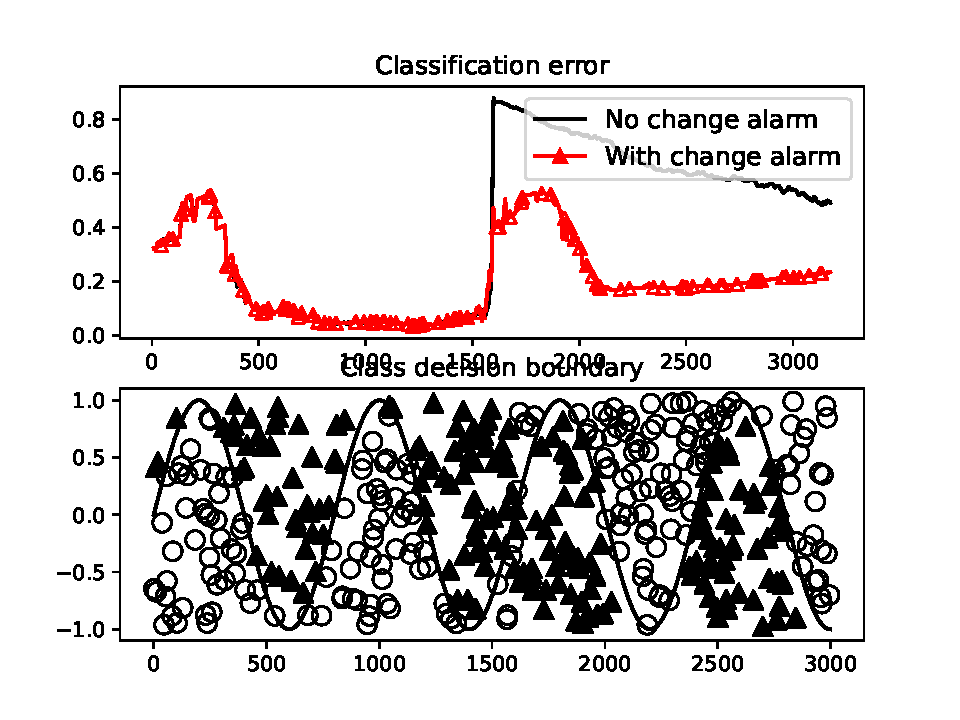
\includegraphics[width=0.7\textwidth]{images/proof_of_concept_dt_sine1}
    \caption{Artificial signal SINE1. Classification.}\label{fig:sine1_example}
  \end{figure}
  Before concept drift error rate decreases according to the statistical decision theory cite{XXX} as model is adaptively retrained. 
  Performance drops after time moment $t$ and detectors alarms the change at the moment $t_1$. 
  Once retrained using relevant data between $t$ and $t_1$, performance becomes better than when updating model continuously.

  Sliding window is a common approach.
  Figure~\cite{fig:art_sig_example} illustrates concept drift phenomenon in regression task when linear regression model is applied to artificially generated signal using sliding window approach. 
  The figure shows predictions and prediction errors.
  % Linear regression artificial signal
  \begin{figure}[!htb]
    \centering
    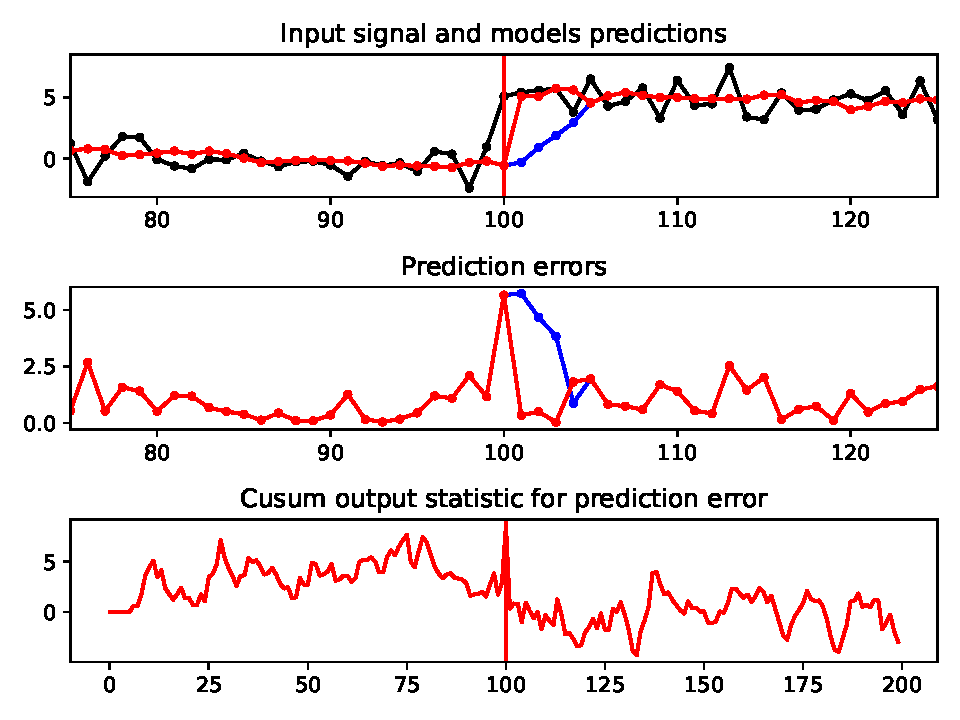
\includegraphics[width=0.7\textwidth]{images/proof_of_concept_linreg_art_sig}
    \caption{Artificial signal example. Linear regression applied in a sliding window. Prediction error with drift detection using Cusum is lower.}\label{fig:art_sig_example}
  \end{figure}

  Figure~\ref{fig:fig7_souza} from~\cite{SouzaRMB20} presents the prequential accuracy of two classifiers: i) Naive Bayes with Drift Detection Method (DMM) (~\cite{gama2004learning}) , and ii) the No-change baseline classifier which predicts the current label to the next event for three datasets. In all cases, the baseline classifier performs better.
  Due that in~\cite{zliobaite2013good} discusses the problem of temporal dependence for the Electricity dataset.

  Continuous model update using sliding or adaptive window is equivalent to the situation when change alarm happens at every time moment.
  \textbf{ROI can help to detect concept drift faster, but since FA is not an issue then we will not observe performance improvement.}
  Figure~\ref{fig:fig28_souza} - FA do not cause performance drop.
  ROI can help to distinguish noisy data from drifts. If model is updated using noisy data then performance will decrease.
  If FA is not due to the noise than it doesn't affect model's performance. 
  One of the main problems with real data sets used for benchmarking concept drift detection methods is an uncertainty about the presence of concept drifts~\cite{SouzaRMB20}.
  If there is false alarm triggering re-training then model will be re-trained using the data between detection and current moment of time instead of the whole sliding window.
  And if it is FA then model's performance will be, most likely, nearly the same.

  % Linear regression CFB 
  \begin{figure}[!htb]
    \centering
    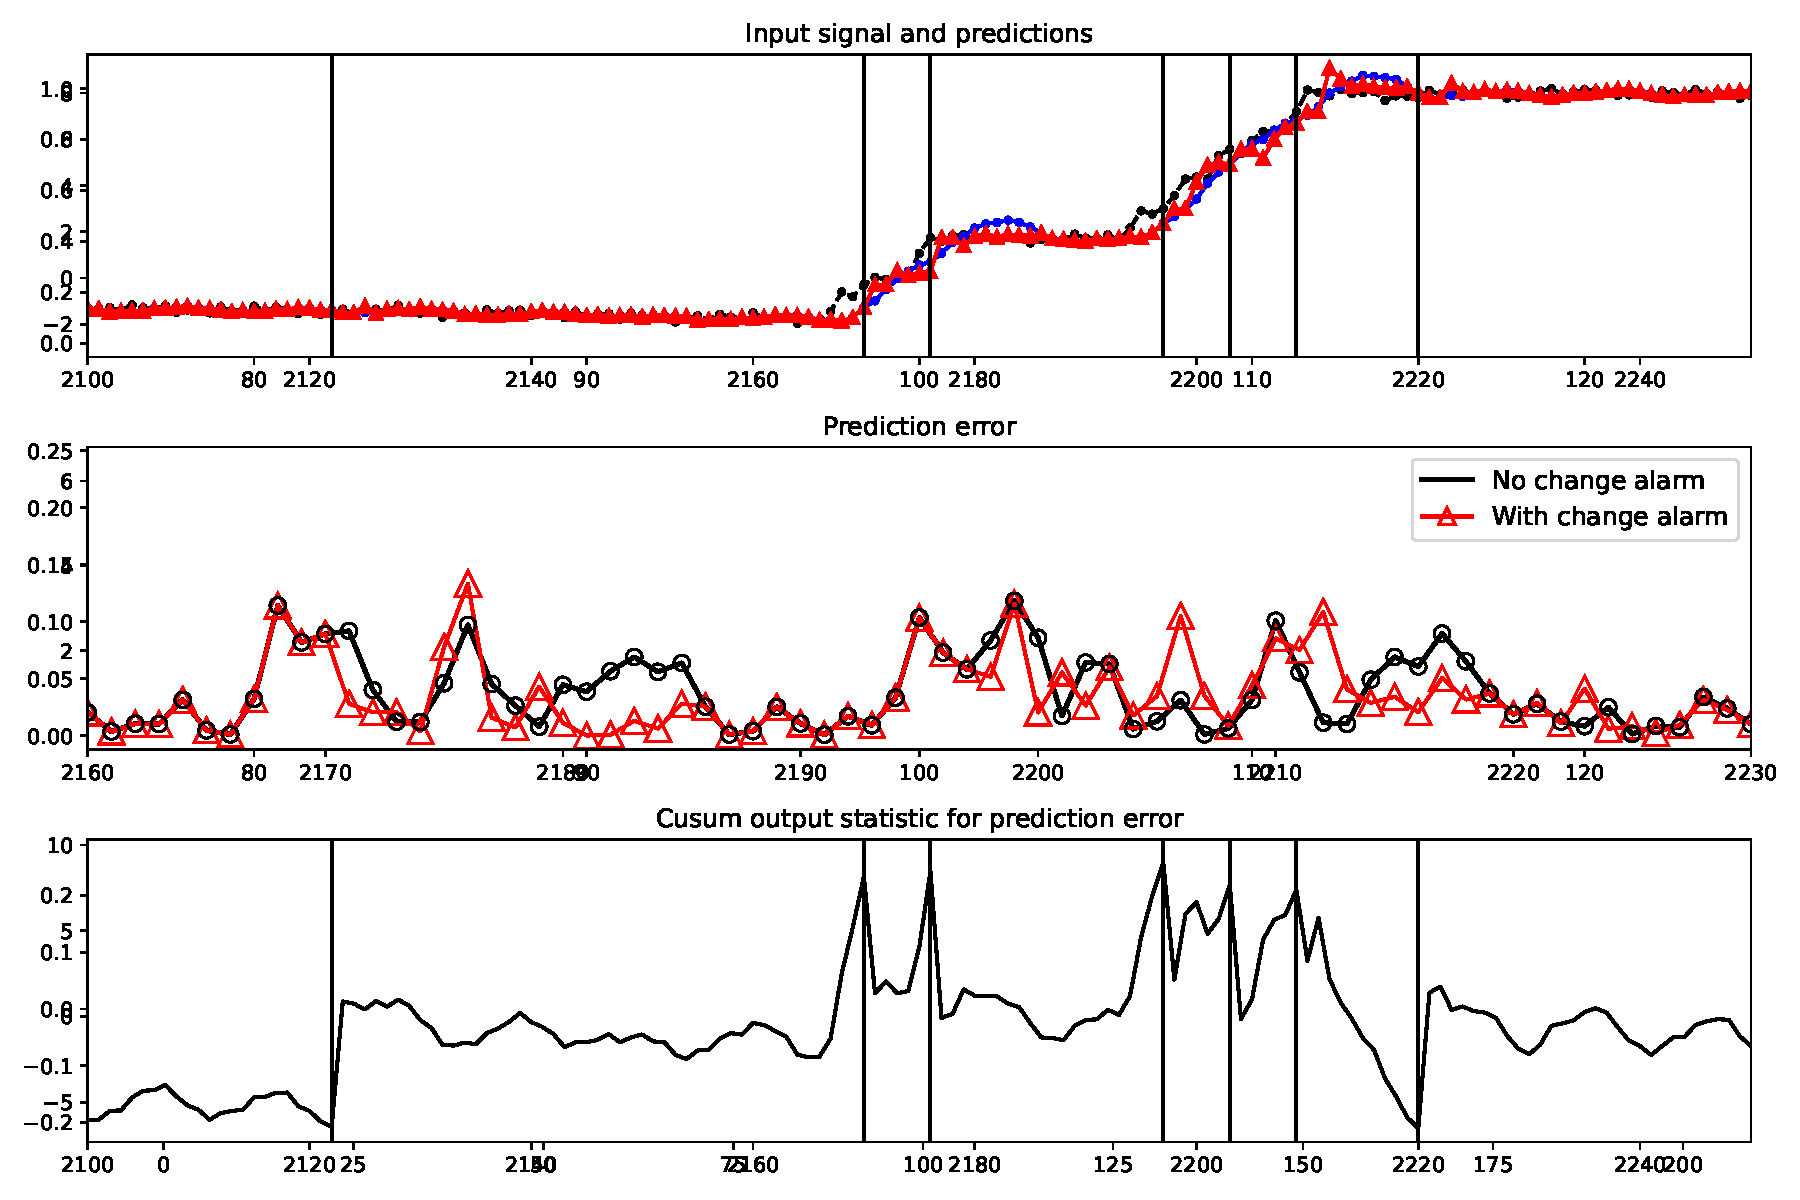
\includegraphics[width=0.7\textwidth]{images/proof_of_concept_linreg_cfb_sig}
    \caption{CFB signal example.  Linear regression applied in a sliding window.  Prediction error with drift detection using Cusum is lower.  FA is not an issue since it doesn't cause any performance decrease.}\label{fig:cfb_sig_linreg_proof_of_concept}
  \end{figure}

  \begin{figure}[htb!]
    \centering
    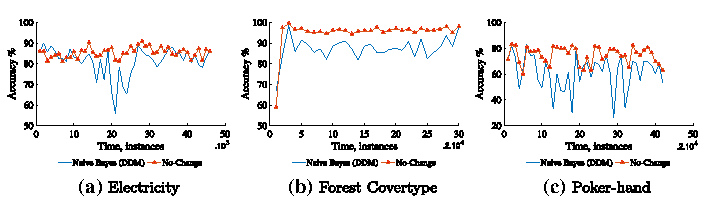
\includegraphics[height=0.15\textheight]{images_cropped/souza_fig7}
    \caption{
  For Electricity dataset, the baseline classifier achieves 85.33\% accuracy while the Naive Bayes with DMM achieves only 81.23\%. For Forest Covertype, the baseline 95.07\% vs 88.04\%. For Poker-hand: 74.51\% vs 61.96\%.
  ~\ref{fig:fig7_souza}
    }\label{fig:fig7_souza}
  \end{figure}

Concept drift occurrence in the insects data set~\cite{SouzaRMB20} is controlled by temperature.
% Sec. 55
  \begin{figure}[htb!]
    \centering
    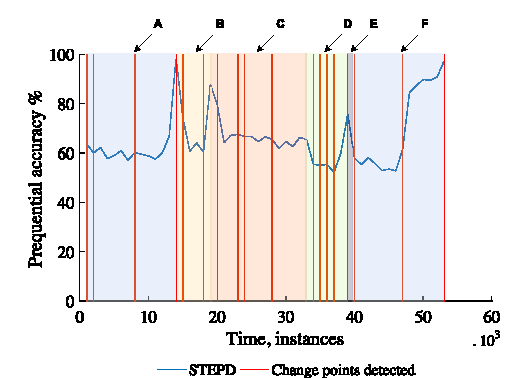
\includegraphics[height=0.4\textheight]{images_cropped/souza_fig28}
    \caption{FA do not cause performance descrease}
    \label{fig:fig28_souza}
  \end{figure}

  \newpage
  \bibliographystyle{unsrt}
  \bibliography{references}
\end{document}
